\documentclass[journal,compsoc]{IEEEtran}
\usepackage[nocompress]{cite}
\usepackage[font=normalsize,labelfont=sf,textfont=sf]{subfig}
\usepackage{graphicx}
\usepackage{arabtex}
%\usepackage{fixltx2e}
%\usepackage{stfloats}
%\usepackage{url}
\usepackage[cmex10]{amsmath}
%\usepackage{array}
%\usepackage{mdwmath}
%\usepackage{mdwtab}
%\usepackage{eqparbox}

%packages that were not copied from the IEEE template - need to check if it is valid to add them
\usepackage{amssymb}
\usepackage{multicol}
\usepackage[linesnumbered]{algorithm2e}

%TODO: Add biography and image for me and for DR. Raid.
%TODO: Check for plagiarism in all the document.

%abbreviations:
% CP: Candidate Segmentation Point
% HF: Horizontal Fragment.
% WP: Word Part
% SSA: Segmentation Selection Algorithms

\begin{document}

\title{Recognition-based Segmentation of On-line Handwritten Arabic Script}


\author{George~Kour,
		Raid~Saabne}

%\markboth{Journal of \LaTeX\ Class Files,~Vol.~6, No.~1, January~2007}%
%{Shell \MakeLowercase{\textit{et al.}}: Bare Demo of IEEEtran.cls for Computer Society Journals}

\markboth{\today}{}

%\IEEEspecialpapernotice{(Invited Paper)}


\IEEEcompsoctitleabstractindextext{
\begin{abstract}
character segmentation has an integral role in many Optical Character Recognition (OCR) systems due to the fact that correctly segmented characters are likely to be recognized correctly. However, Correct and efficient segmentation of Arabic text into characters is considered to be an essential problem. The cursive and unconstrained nature of the Arabic script in both printed and handwritten forms anneals the segmentation task. The Arabic script is composed of strokes which represent a single letter, multiple connected letters or diacritics. This paper proposes a novel on-line strokes-level recognition-based segmentation technique of Arabic script. The advantage of our approach is that the most time consuming procedures are performed while the stroke is being scribed. The system consists of three stages. The first stage, which requires the most calculation effort, is performed whilst the stroke is being written and involves over-segmentation using topological and directional local features and recognition-based scoring of adjacent combinations of sub-strokes that induced by the proposed segmentation points. The second stage contains filtering of the topologically invalid segmentation points. The last stage involves several segmentation points selections algorithm which determines the best subset of segmentation points. The system has been designed and tested using the ADAB Database. Promising results were obtained without using context help.
\end{abstract}
\begin{IEEEkeywords}
Arabic Handwriting Recognition, Arabic Script Segmentation, Arabic Strokes Segmentation, On-line Text Recognition
\end{IEEEkeywords}
}
\maketitle

\IEEEdisplaynotcompsoctitleabstractindextext

\section{Introduction}
\date
\IEEEPARstart{H}{andwriting} remains the most used mean of communication and recording of information in the daily life. Therefore, a growing interest in the on-line character recognition field has taken place in the recent years. Handwriting recognition can be categorized into two main fields: off-line and on-line. In the off-line script recognition, a digital image containing text is fed to the computer and the system attempts to convert the spatial representation of the letters into digital symbols \cite{al2011online}. On the contrary, on-line handwriting recognition refers to the situation where the recognition is performed concurrently to the writing process. Approaches for script recognition are usually classified into two types: 1.The holistic approach \cite{biadsy2011segmentation} and 2.the analytic approach \cite{abdulla2008off, sari2002off, Dinges2011, elanwar2012unconstrained}. The holistic approach considers the global properties of the written text while the analytic approach involves segmentation and classification of each part of the text.  In the holistic approach, the recognition system needs to be trained over all words in the dictionary, while it is possible for small vocabulary of words; this is not feasible for large vocabularies (20,000 words or more). Since each word is constructed from a subset of the character alphabet, it is much more efficient to classify words using the analytic approach \cite{elanwar2012unconstrained}.\\

The Recognition of Arabic handwritten script is an important field due to the language widespread. The Arabic language is spoken by more than 230 million people around the world and it is written by more than 100 million people \cite{al2011online}. The Arabic language contains many different dialects used for nearly all everyday speaking situations however the formal standardized language, found mostly in writing or in prepared speech, is common. Approximately 25 languages have adopted the Arabic writing system with some changes. Thus the ability to segment and recognize Arabic script would have a significant academic and economic impact. Nevertheless, the Arabic script recognition is at early stage in relation to the script recognition of Latin, Chinese and Kanji which has been a focus of study in the last decade and achieved an impressive recognition rates. 
Character Recognition of the Arabic script is more complicated than other languages such as English and Chinese due to the peculiarity nature of the Arabic script that include cursiveness, context sensitive shapes and overlapping \cite{razzak2010locally}. Other reasons this lagging include several technical reasons such as lack of funds, text database and dictionaries absence, etc.\cite{zeki2011segmentation}.\\

The Arabic language is written right to left in a cursive manner in both handwritten and printed forms. Most Arabic letters has four main body shapes: Isolated, Medial, Initial and Final, while other letters have two main body shapes: Isolated and Final. An occurrence of two shapes letters inside a word will lead to a split of the body into two or more parts, called Word-Parts (WPs). Within the WP, the letters are connected in both handwritten and printed. Different letters may share the same body and only differ by additional strokes and dots named diacritics as can be seen in figure \ref{fig:same_body_letters}. In many cases, Arabic WPs which are connected when printed, are written in multiple strokes in handwritten form as can be seen in figure \ref{fig:kmbot}. \\

\begin{figure}
\centering
\renewcommand{\arraystretch}{2}
%{\footnotesize
\begin{tabular}{| c | c | c | c |}
\hline
\RL{.h} \RL{j} \RL{x}& \RL{r} \RL{z} & \RL{f} \RL{q} & \RL{`} \RL{.g} \\
\hline
\RL{.t} \RL{.z} & \RL{s} \RL{^s} & \RL{.s} \RL{.d} & \RL{b} \RL{t} \RL{_t} \\
\hline
\end{tabular}
\caption{Arabic Letters groups having identical main body.}
\label{fig:same_body_letters}
\end{figure}

Wrong segmentation of a word is likely to result in wrong recognition. The other way around is also valid when it comes to recognition-based segmentation techniques, i.e. a firm recognition system improves the segmentation precision. Several segmentation approaches have been proposed in the literature for Arabic OCR. Yet, correct and efficient segmentation of Arabic text is an unmet need and considered to be a challenging and a fundamental problem even for off-line printed text. A common approach that is followed by many researchers is over-segmentation of the text and validating each such candidate segmentation point by extracting feature vectors representing the segmented parts to some classifier or rules based engine \cite{daifallah2009recognition}.\\

Methods used by segmentation-based approaches can be mainly classified into two: Dissection and Recognition-Based Segmentation. Dissection techniques learn the characteristic of the segmentation point and attempt to find appropriate candidate points. For instance, local minima in the upper or lower contour is commonly used for segmenting English cursive script. Other widely used feature that characterizes a segmentation point is the low slope of its local environment. The dissection of words into segments do not necessarily correspond to exactly one character per segment, however it could segment the words into components called graphemes, which are a combination of two or three letters, or a part of a letter. The relationship between graphemes and letters is applied in a later phase. The recognition-based techniques operate quite differently. The method includes using a moving window with a predefined width which breaks the word into many overlapping pieces without regard to its content and the attempts to classify those sub-components to find points of interest or trajectories. An iterative or parallel scanning of the words followed by a recognition method is used to search for "satisfactory" classification scoring for joint sub-components usually by generating a lattice of all or many possible combinations. The final decision is determined by the best path through the lattice. While avoiding using complex dissection methods, such techniques rely heavily on the classifier accuracy \cite{casey1996survey}. \\

In this paper we propose a novel approach which performs segmentation and recognition in the strokes level. We combine both holistic and analytic techniques for recognizing open dictionary Arabic on-line script. In section \ref{sec:related_word} we mention related studies done in the field of on-line Arabic recognition. The proposed approach is described in details in section \ref{sec:approach}. Results are shown in the section \ref{sec:results}. We present our plans for future work in section \ref{sec:future_work}.

\begin{figure}
\centering
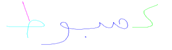
\includegraphics[width=6cm]{./figures/kmbot_color}       
\caption{The Tunisian city name kambot \RL{kmbw.t}. It contains two word parts (\RL{kmbw} and \RL{.t}). The main body of the first WP is written using three strokes: 1. The letter \RL{k-} 2. The connected letters combination \RL{-mbw} 3. The additional dot of the letter \RL{-b-}. The second WP contains only a single letter (\RL{.t}) and is written using two strokes, the main body and an additional stroke.}
\label{fig:kmbot}
\end{figure}

\section{Related Work}
\label{sec:related_word}
A rules-based system for off-line Arabic handwritten word segmentation was presented by Abdulla et al. in \cite{abdulla2008off}. Their method is based on extracting features of pixels lying on the upper contour. The freeman chain coding scheme was used to find the coordinates of the contour. After calculating the slope of the upper contour pixels, the direction of pairs of adjacent coordinate were marked by '+' or '-'. Segments were combined to formulate bigger decisive segments (DS). Then, a set of possible segmentation point are nominated from the '+' marked segments. These segmentation points were evaluated using a certain rules to find the final segmentation points (FSP). The system was tested on the demo version of IFN/INIT described in \cite{pechwitz2002ifn} , and their own AHD/AUST database.\\

Randa et al. proposed a two stage word segmentation system of on-line Arabic handwritten text based on Hidden Markov Model (HMM) in \cite{elanwar2012unconstrained}. In the first stage, segmentation points were nominated by a simultaneous segmentation-recognition method using HMM. The proposed segmentation points were validated by a rules-based stage. Additional strokes were removed and not taken into consideration in both parts. The system was tested using a self-collected database (OHASD) that was described in \cite{elanwar2010ohasd}.\\

Another method described in \cite{sari2002off} by Sari el al. proposed a method for off-line Arabic Word parts segmentation based on the topological characteristics of the word contour. A contour following  algorithm was applied to achieve a smoothed sequence of the X-Y coordinates of the outer contour. Local minima were identified in the lower contour to nominate segmentation points. Then, a rules based engine was employed to identify valid segmentation points. The system was evaluated using a small database that contained 100 handwritten Arabic words sampled.\\

A segmentation based recognition approach was described by Laslo Digness et al. in \cite{Dinges2011}. Their method is based on dividing the word to smaller pieces which afterwards segmented into candidate letters and then classified into letter classes using statistical and structural features. Decisive tree were used to reduce the number of potential classes; neural networks to compute weights for all statistical features. The output of this process was used as input for a k-NN classifier to obtain the final recognition.\\

Khaled Daifallah et al. in \cite{daifallah2009recognition} proposed a method for on-line Arabic handwritten words recognition. Their method operates on the stroke level. It is based on segmentation-based recognition which contain several stages. The first stage proposes over-segmentation of the stroke. The segmentation points are selected by locating semi-horizontal lines moving from right to left. In a latter phase, a portion of the segmentation points is filtered out by applying on a certain set of rules. Then, HMM is used to classify the sub-strokes to letters using Hu feature. The candidate and its scoring letters results were used to determine the best set of segmentation points. \\

Eraqi and Abdelazeem \cite{eraqi2012new} suggested splitting the Arabic handwriting off-line data into basic graphemes based on the geometric properties. The image was skeletonized and using Douglas-Peuker lines simplification algorithm, linear piecewise linear curves were obtained. Diacritics and noise segments that often appear in the binarized image were removed. Horizontal segments were found by calculating the angle between the skeleton lines of the shape and the x-axis. Linear regression was used to find the baseline and all least fitting segmentation points filtered out. Then, a rules based procedure was applied to extract the graphemes corresponding to the final segmentation points were extracted.    

\section{Approach}
\label{sec:approach}
Our approach employs both rules-based dissection and recognition-base segmentation techniques. The main idea is to segment a stroke while being scribed. A stroke is a subcomponent of a WP that spans from the pen down event to the corresponding pen up event. We assume that the main body of a letter is contained entirely in a single stroke, i.e. no letter span over multiple strokes. This assumption is valid for the majority of Arabic  handwriting styles. The motivation behind this method is based on the intuition that the most basic structure that can be recognized by a human reader is the stroke. Thus being able to correctly segment and recognize the content of a stroke will vastly facilitate the Arabic script recognition problem. In this work our objective is to maximize the correct segmentation rate while maintaining low complexity and high performance of the system. Maximizing the recognition rate is a secondary objective. 
The proposed technique describes a general concept of ongoing strokes segmentation. The decoupling between the different components and sub-components in the system enables different alternatives techniques to be integrated easily.\\ 

Below, a digest of the three main stages of our approach: 

\textbf{Stage 1.} Segmentation points in the Arabic script reside, in most cases, in horizontal handler that joint a pair of connected letters. These handlers are mostly horizontal, directed right to left and located near the baseline. In this stage the system attempts to identify horizontal fragments (HF) in the written stroke, nominate candidate segmentation points (CP) and give scoring to the sub-strokes that are imposed by the CPs. The scoring is saved in a matrix-like data-structure and represent the resemblance of the sub-stroke to some Arabic letter. This stage is activated continuously after reception of small and constant number of points. 

\textbf{Stage 2.} The CPs are investigated and invalid candidate points are filtered out. Then, a scoring correction process is invoked to adjust the scoring of the sub-strokes using several heuristics.

\textbf{Stage 3.} Using the scoring of the sub-strokes, a collection of algorithms are employed to select the final set of segmentation points.

A high level description of the system flow can be seen in figure \ref{fig:system_flow}. Detailed explanation on each stage is provided in the subsections below.

\begin{figure}
\centering
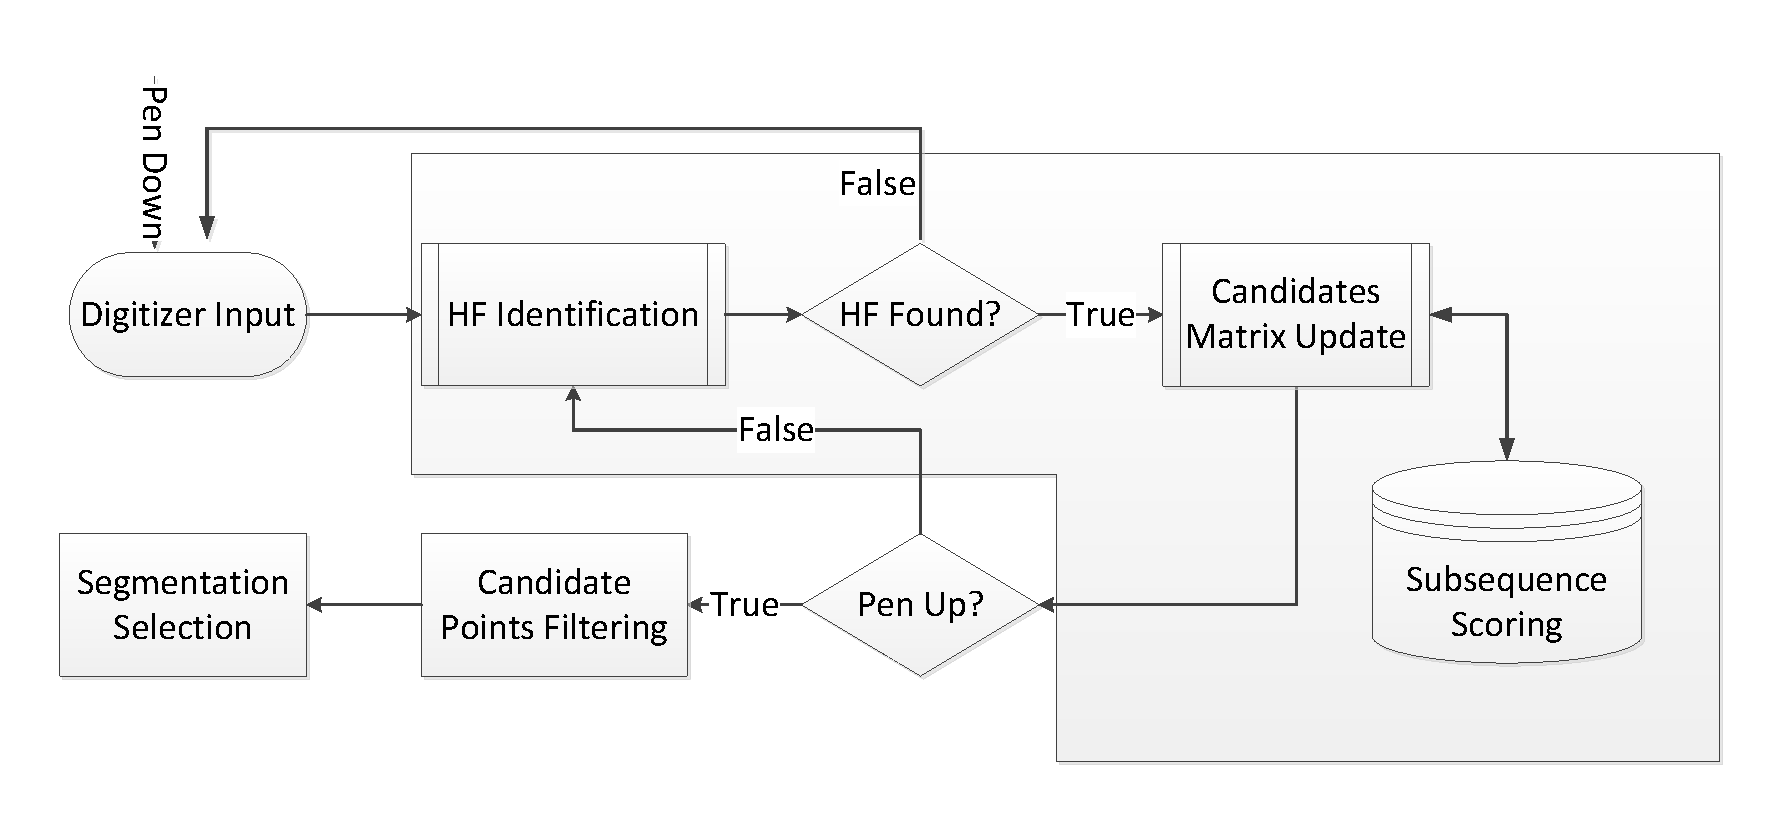
\includegraphics[width=9.5cm]{./figures/system_flow}
\caption{High level system flow. The first stage is multi-phase and contain three subcomponent. }
\label{fig:system_flow}
\end{figure}

\subsection{First Stage: Segmentation points nomination and sub-strokes scoring}
\subsubsection{Horizontal Fragment identification}
The goal of this process is to identify HFs in the written text. HFs of the Arabic word \RL{jbl} (Jabal) can be seen in figure \ref{fig:horizontal_fragments} .Once an HF is detected, its medial point is marked as a CP. A HF is a subsequence of the stroke having the following properties: 
\begin{enumerate}
\item relatively straight
\item low slope
\item directed right to left 
\end{enumerate}
The method described below attempts to identify the largest possible HF and disregard small horizontal regions that are usually caused by the imperfection of the digitizer. The HF identification is performed by spotting it's start and the end points.
Once an HF is identified, the medial point of the HF is nominated as a CP.
A point $p_{i}$ is named a "horizontal point" if the slope of the line $\overline{p_{i-1}p_{i}}$ if $\frac{\Delta x}{\Delta y}\leq0.6$. This parameter was tunes empirically. The same exact value for this parameter was found independently in \cite{daifallah2009recognition} which strengthen our confidence of our finding.\\
To reliably calculate the slope value despite the noisy data obtained by the digitizer, a preprocessing step is needed. The preprocessing include down-sampling to the half of the sample points of the original trajectory. \emph{which resampling algorithms was used?}
Once the first low slope point is recognized, the algorithm sets this point as a HF starting point. Every next low slope point is marked as "Last Seen Horizontal point" Until a high slope point is obtained. The point lastly marked as "Last Seen Horizontal point" is set to be an "Ending Horizontal point".\\

The nominated segmentation points in this stage is an over-segmentation of the stroke. It is important to note that this process is imperfect and may result in finding fragments that would not be classified as HF by a human performing the same task. As can be seen in figure \ref{fig:candidate_in_no_horizontal}, this stage may find very small HF that may result from the digitizer imperfections. However, it is important not to apply too many restrictions such as imposing a minimal length on the HF since while extra CP can be easily filtered out in a later phase when the entire stroke is available, failing to find a CP can't be recovered. In our experiments we observed that more than 99\% of true segmentation points were included in the over-segmentation imposed in this stage.\\

In order to avoid the case where HFs are over identified frequently, we have employed HF merging method that operates as follows: At every HF identification, we calculate the complexity measure of the stroke (a measure that quantify the cursiveness of the trajectory - described in section \ref{subsec:scm}) from the previous HF and if the result is small, the two HF is merged into a single HF. The reason for executing the HFs merging operation while the stroke is being written and not waiting to a later stage is that over identification of HFs may result in extreme over-segmentation, and reduce the performance and accuracy of the CPs selection stage.

\begin{figure}
\centering
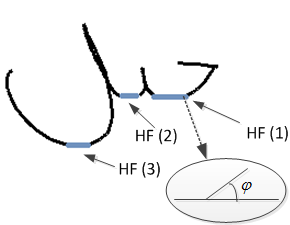
\includegraphics[width=5cm]{./figures/horizontal_fragments}
\caption{Horizontal Fragments [HF] of the word \RL{jbl}(JABAL)}
\label{fig:horizontal_fragments}
\end{figure}

\begin{figure}
\centering
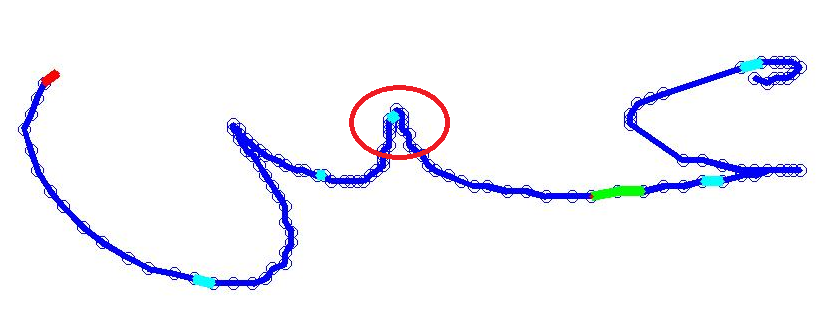
\includegraphics[width=6cm]{./figures/candidate_in_no_horizontal}
\caption{The main body of Arabic word \RL{`yn}. CPs are colored in cyan. The green areas ensigns that HFs merge has taken place. Three types of false CPs can be seen: 1. A CP at the beginning of a stroke. 2. A candidate point that do not reside on a HF. 3. A CP on the valley of the letter \RL{-n}. }
\label{fig:candidate_in_no_horizontal}
\end{figure}

\subsubsection{Sub-strokes scoring}
A stroke $S$ is represented by a sequence of points on the 2-dimensional space, $p_{i}=(x,y)$ 
\begin{equation}
S=\{p_{i}\}_{i=1}^{n}
\end{equation}
Let $KP$ (Key Points) be zero based ordered set containing the CPs found in the previous sub-stage and that also include the first and the last point of the stroke $S$. Assuming $L$ CPs were found in the stroke $S$, $KP$'s definition is as follows: 
\begin{equation}
KP_{i} =\begin{cases}    1		, & \mbox{if } i=0 \\
							   CP_{i}	, & \mbox{if } 1\leq i \leq L \\
							   n    , & \mbox{if } i=L+1 
			\end{cases}				
\end{equation}
A sub-stroke $S_{i}^{j}$ is a sub-sequence of the stroke $S$ that starts at $KP_{i}$ and ends at $KP_{j}$, formally:
\begin{equation}
S_{i}^{j}=(p_{k})_{k=KP_{i}}^{KP_{j}}; i<j
\end{equation}
The Sub-sequence Scoring Matrix $D\in\mathbb{R}^{n\times n}$ contains the resemblance scoring obtained by the classifier to the corresponding sub-strokes in $S$, i.e:
\begin{equation}
D(i,j)=Score(S_{i}^{j})
\end{equation}
It is clear that $D$ is an upper triangular matrix. In Order to maintain good performance as well as high segmentation accuracy, we added a locality constraint to avoid marginal segmentation. That is, we only calculate a narrow band of the $D$ matrix above the main diagonal. Assume the band width is equal to $B$.
\begin{equation}
D(i,j)=\infty \Leftrightarrow j \leq i \vee j-i>B 
\end{equation}
We assume that sub-strokes which represent a letter will achieve better resemblance scoring, i.e. $D(i,j)$ value will be smaller relative to other sub-stroke. The matrix $D$ is calculated while the stroke is being scribed. Once a new CP is identified a new row and column are added to the matrix $D$. 
The number of cells that will be calculated at each new CP is $B$ (all located in the new column).\\

\begin{figure}
\centering
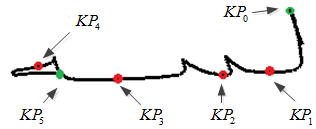
\includegraphics[width=7cm]{./figures/candidate_points}
\caption{Key Points of the word  \RL{lbyh}. The first and last key points are colored in green. The red points are the candidate points}
\label{fig:candidate_points}
\end{figure}

The sub-strokes scoring system is described in depth in \emph{[my paper]}. For the sake of completeness, here we will outline the main idea of the classification system. The classifier uses Shape Context to extract the pattern feature, then Earth movers Distance embedding technique descried in \cite{shirdhonkar2008approximate} to project samples of the Arabic letters to a high dimensional $L_{1}$ space. A combination of Principle Component Analysis (PCA) and Linear Discrimination Analysis (LDA) is used to reduce the samples dimensionality and k-NN are found using k-dtree. The exact resemblance score is determined by a minimum score that is given by a predefined linear combination of the $L_{1}$ distance in the embedding space and Sokoe-Chuba DTW.\\

The scoring system contains four databases, one for each letter position. It receive a sequence and a position (Ini, Mid, Fin and Iso).
As mentioned earlier a stroke spans from the mouse down to the mouse up event. 
A stroke may contain a full or a partial WP and can be composed of the following letter positions: 
\begin{multicols}{2}
\begin{itemize}
    \item $Iso$
    \item $Ini,Mid^{*}$
    \item $Mid^{+}$    
    \item $Mid^{*},Fin$
    \item $Ini,Mid^{*},Fin$
\end{itemize}
\end{multicols}
In the above list, the $^{+}$ notation represents one or more occurrences and $^{*}$ notation represents zero or more occurrences.

In order to maximize performance and accuracy, the system should attempt to look for the letter label and scoring in the smallest number of databases. To make the following explanation clearer let us define the following four types of sub-sequence:
Let $S$ be a sequence which contains $L$ candidate points: 
\begin{itemize}
	\item \textbf{$\alpha$ subsequence:}  A sub-sequence $S_0^k$ where $ 1\leq k < L+1$. It may contain an initial or medial letter only.
	\item \textbf{$\beta$ subsequence:}  A sub-sequence $S_m^k$ where $m \geq 1 \wedge m< k \leq L$. It may contain a medial letter only.
	\item \textbf{$\chi$ subsequence:}  A sub-sequence $S_m^{L+1}$ where $m \geq 1$. It can contain only a medial or final letter.
	\item \textbf{$\delta$ subsequence:} A sub-sequence $S_0^{L+1}$. It can represent letter in any position.
\end{itemize}
The $D_p$ matrix in equation \ref{eq:positions_matrix} below relates between the cell location in the $D$ matrix and the database that the scoring system will look for the best matches. It is important to note that the $D$ matrix is filled while the stroke is being written, thus, the system has no knowledge on how many candidate points the stroke will end up having or when the writer will end the stroke. 
\begin{equation}
D_{p}=
\left( 
\begin{array}{ccccccc}
\infty 	& \alpha & \alpha & \alpha  & \cdots & \alpha & \delta \\
\infty  & \infty  & \beta   & \beta   & \cdots  & \beta  & \chi    \\
\infty  & \infty  & \infty   & \beta   & \cdots  & \beta  & \chi    \\
\vdots & \vdots & \vdots  & \vdots & \ddots  & \vdots & \vdots \\
\infty  & \infty  & \infty   & \infty   & \cdots  & \beta  & \chi    \\
\infty  & \infty  & \infty   & \infty   & \cdots  & \infty  & \chi    \\
\infty  & \infty  & \infty   & \infty   & \cdots  & \infty  & \infty \end{array} \right)
\label{eq:positions_matrix}
\end{equation}

For each subsequence, the recognition system returns a set of K potential letters candidates, with their resemblance scoring (in our implementation $K=3$). In the current implementation we consider only the candidate with the best (minimal) scoring, however, any function taking into consideration the scoring returned by the classifier for all the candidate can be used to determine the final scoring of the cell.
Figure \ref{table:substrokes_demo} visually demonstrates the Subsequences that is scored for each cell in matrix $D$.


\begin{figure}
\centering
\renewcommand{\arraystretch}{2}
\begin{tabular}{| c |c | c | c| c | c | c |}
\hline
 $KP_i$ & $0$ & $1$ & $2$ & $3$ & $4$ & $5$\\ 
\hline
$0$
   & N/A
   & \subfloat{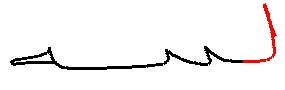
\includegraphics[width=0.8cm]{./figures/substrokes/L}}
   & \subfloat{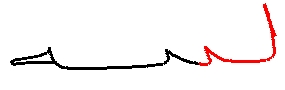
\includegraphics[width=0.8cm]{./figures/substrokes/LB1}}
   & \subfloat{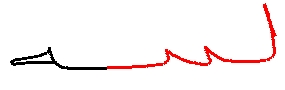
\includegraphics[width=0.8cm]{./figures/substrokes/LB1B2}}
   & N/A & N/A \\
\hline
$1$
   & N/A & N/A
   & \subfloat{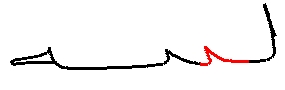
\includegraphics[width=0.8cm]{./figures/substrokes/B1}}
   & \subfloat{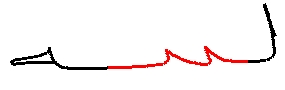
\includegraphics[width=0.8cm]{./figures/substrokes/B1B2}}
   & \subfloat{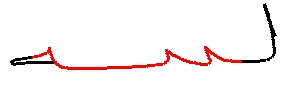
\includegraphics[width=0.8cm]{./figures/substrokes/B1B2H1}}
   & N/A \\
\hline
$2$
   & N/A  & N/A & N/A
   & \subfloat{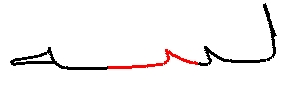
\includegraphics[width=0.8cm]{./figures/substrokes/B2}}
   & \subfloat{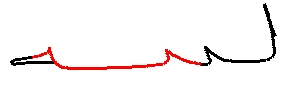
\includegraphics[width=0.8cm]{./figures/substrokes/B2H1}}
   & \subfloat{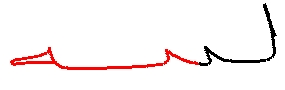
\includegraphics[width=0.8cm]{./figures/substrokes/B2H}} \\
\hline
$3$
   & N/A & N/A & N/A & N/A
   & \subfloat{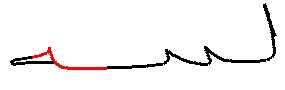
\includegraphics[width=0.8cm]{./figures/substrokes/H1}}
   & \subfloat{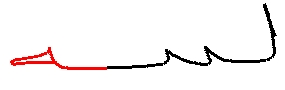
\includegraphics[width=0.8cm]{./figures/substrokes/H}} \\
\hline
$4$
   & N/A & N/A & N/A & N/A & N/A
   & \subfloat{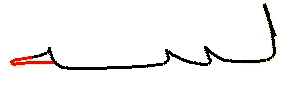
\includegraphics[width=0.8cm]{./figures/substrokes/H2}}\\
\hline
$5$
   & N/A & N/A & N/A & N/A & N/A & N/A \\
\hline
\end{tabular}
\caption{Visual demonstration of subsequences of the word shown in figure \ref{fig:candidate_points}}
\label{table:substrokes_demo}
\end{figure}

\subsection{Second  Stage: Candidate points sieving and scoring correction}
In this stage we eliminate redundant segmentation points found in the over-segmentation process of the previous stage. The elimination is based on the following rules:

\begin{itemize}
	\item[] \textbf{Rule 1:} Inner Segmentation point lies close to the baseline. 
	\item[] \textbf{Rule 2:} Segmentation points do not reside in loops.
	\item[] \textbf{Rule 3:} A sub-stroke length/area is proportional to the stroke/length of the containing stroke.
\end{itemize}

The baseline is proved to be an important piece of information for both segmentation and recognition in both on-line and off-line handwriting recognition. In the recognition process, it plays a role in determining the type of the diacritic according to their position from the baseline (above or under). In this work we use the baseline to determine if a candidate point is a possible segmentation point according to its distance from the baseline. We don't need to determine the exact position of the baseline since all we need to do is to make sure that the candidate points are in a reasonable distance from the baseline.
The second rule is clear since in most writing styles, segmentation point do not reside inside a loop.
The third rule's goal is to avoid high scoring resulted for discordant scaling of the letters; a scoring correction should be employed. It aims to reduce the effect of scaling problem. To illustrate the discordant scaling problem, see figure below. The suffix of the letter \RL{d} is very similar to the letter \RL{-a}. The only way to visually discriminate between them is by comparing the scaling of this suffix to the whole stroke dimensions. Thus this phase refines the recognition results according the subsequence scale in accordance to the sequence scale. We have penalized sub-strokes that are disproportional to the stroke size by multiplying the score of each sub-stroke with a Gaussian normalized by the stroke area/Length.
In some cases candidate segmentation points are incorrectly nominated on areas that are not horizontal, this is caused from the fact that the nomination is done while the word is being scribed, and our filtering algorithm should be corrected to handle this case.

\emph{[Talk about the scoring correction procedure]}.

In several cases we encountered candidate points that reside on the same horizontal fragment. \emph{[why does it happen?]}. We filter out this redundant candidate points in the nomination process and do not wait till this filtering phase. The reason is that since we calculate a narrow band of the Scoring matrix, leaving the impermissible candidate points will result in low performance since highly over segment the word will cause also the system to miss letters because we calculate only a portion a narrow band of the scoring matrix. If such case is identified by the nomination algorithm the medial point between the adjacent candidate points is taken.

\subsubsection{Baseline detection}
Once the entire stroke is available, a baseline detection algorithm is activated only if more than four CPs were detected. The reason for this threshold is to prevent the baseline detection procedure to be activated on small strokes where the baseline can't be reliably determined. To find the handwritten stroke's baseline, the vertical density histogram of the re-sampled stroke is used. The $\Delta y$ of the stroke is calculated and partitioned to 10 intervals, then the center of the of the most common interval is calculated $I_{max}$. A candidate point $CP$ is filtered out if the following holds:
\begin{equation}
|Y(CP)-I_{max}|>2*max(|I|,0.15) 
\end{equation}
Where $Y(\cdot)$ is the y coordinate of the CP and $|I|$ is the length of the interval. 
Filtering out CPs that are relatively far from the baseline has proven to be very effective in eliminating false CPs that reside on valleys of several letters, such as \RL{q}, \RL{s} and \RL{n}, in the their final and isolated positions. These CPs are usually challenging because they tend to be included in the final set of candidate points if not filtered out. An example can be seen in figure \ref{fig:candidate_in_no_horizontal}, note the candidate point (cyan) inside the last letter \RL{-n}. 

\subsection{Third Stage: Segmentation Selection}
The goal of this phase is to select the best segmentation points set among the candidate segmentation points. It is done by finding a segmentation path in $D$ having best scoring possible. 
 
A segmentation path $\pi$ with in subsequences scoring matrix $D^{m\times n}$ is a sequence of cells in the following form: $\pi=(1,a_{1}),(a_{1},a_{2}),(a_{2},a_{3}),...,(a_{L},n)$. The path defines a unique segmentation. The segmentation set is the following set:  $\{a_{i}\}_{i=1}^L$.

Formally, the a path should have the following properties:
\begin{enumerate}
\item First cell: $\pi_{1}=(1,\_)$
\item $ \forall (1<k<L): \mbox{ if } \pi_{k-1}=(i,j) \mbox{ then } \pi_{k}=(j,r) \mbox{ s.t } j<r<n$
\item Last cell: $\pi_{L}=(\_,n)$
\end{enumerate}
The scoring of the path $\pi$ is defined as follows:
\begin{equation}
\Pi = \Sigma_{i=1}^{L}{D(\pi_{i})}
\end{equation}

Several segmentation selection algorithms (SSAs) are proposed in this work for finding the best segmentation path, i.e. the path $\pi$ with the smallest $\Pi$ possible, which presumingly, represent the correct segmentation of the stroke $S$. The output of all the SSA that will be described is a set, named \emph{Final Segmentation Points} $FSP$, which contain indexes of the final segmentation points in $KP$. The first point of the stroke (namely, $KP_1$ and $KP_n$) not included in FSP.
The first two proposed algorithm were given the names \emph{Forward Segmentation Selection} (FSS) and \emph{Backward Segmentation Selection} (BSS) which operate is pretty similarly. A pseudo-code of FSS can be seen in Algorithm \ref{alg:fss} below. It operates sequentially on the Candidate points set (CPS). Starting from the first point in the stroke it tries to find the next best segmentation point by selecting the subsequence $S_i^j$ having the best scoring value as can be seen in line 5.  BSS (see Algorithm \ref{alg:bss}) operates similarly, However it starts from the end of the stroke toward the beginning. The weakness of the these two algorithms is that FSS tended to under-segment the suffix of the stroke and BSS tended to under-segment the prefix of the stroke.   

\begin{algorithm}
$i=0$\;
$sum=0$\;
$FSP = \emptyset $\;
\While{$i<L+1$}
{
	$j = \mathop {\arg \min }\limits_k \left( {D\left( {i,k} \right)} \right)$\;
	$FSP = FSP \cup \left\{ j \right\}$\;
	$sum = sum + D\left( {i,j} \right)$\;
	$i=j$\;
}
\caption{Forward Segmentation Selection (FSS)}
\label{alg:fss}
\end{algorithm}

\begin{algorithm}
$i=L+1$\;
$sum=0$\;
$FSP = \emptyset $\;
\While{$i>0$}
{
	$j = \mathop {\arg \min }\limits_k \left( {D\left( {k,i} \right)} \right)$\;
	$FSP = FSP \cup \left\{ j \right\}$\;
	$sum = sum + D\left( {i,j} \right)$\;
	$i=j$\;
}
\caption{Backward Segmentation Selection (BSS)}
\label{alg:bss}
\end{algorithm}

To overcome the aforementioned drawback of FSS and BSS a third SSA was proposed and was given the name \emph{Backward-Forward Segmentation Selection} (BFSS) described in Algorithm \ref{alg:bfss}. It is a combined version of both FSS and BSS. BFSS operates from the sides of the stroke toward the center. While the set of the unselected candidate points is not empty, in each iteration the algorithm selects two candidate points to include to the $SSP$ set. The selection of a the next candidate point is done by finding the next best sub-stroke, i.e. the cell with the least scoring that start with the current selected segmentation point.
When a candidate point is added to the $SSP$ set "cleaning" operation is done to remove all the preceding candidate points that were not selected. For example, if $KP_{i}$ was selected in the previous iteration and the current iteration $KP_{i+2}$ is selected, all cells related to $KP_{i+1}$ will be set to $\infty$ in the matrix $D$ to avoid this candidate point to be selected in a later iteration. Also all cells that represent a sub-stroke starting from candidate point $KP_i$ or ending in $KP_{i+2}$ will be set to $\infty$. Lines 7-10 handles the the segmentation of the left side of the word and the lines 11-15 handles the right side of the word. This algorithm is an combination of two algorithm we were suggested, the first that operates forward to select the segmentation path and the other is backward algorithm that start from the end of the word toward the start. However, we noted that the forward algorithm tended to under-segment the suffix of the stroke, i.e. missing true segmentation points and the other tended to under-segment the prefix of the stroke.  

\begin{algorithm}
$cp_{a}=1$\;
$cp_{b}=n$\;
$sum = 0$\;
$CPS = KP\setminus\{1,n\}$\;
\While{$CPS \neq \emptyset$}
{
	$cp_{a,next} = \mathop {\arg \min}\limits_k (D(cp_a,k))$\;
	$FPS = FPS \cup \{cp_{a,next}\}$\;
	$CPS = CPS\setminus\{cp_{a,next}\}$\;
	$sum = sum + D(cp_a,cp_{a,next})$\;
	$UpdateMatrix(D,cp_a,cp_{a,next})$\;
	$cp_{a}=cp_{a,next}$\;
	
	$cp_{b,next} = \mathop {\arg \min}\limits_k (D(k,cp_{b,next}))$\;
	$FPS = FPS \cup \{cp_{b,next}\}$\;
	$CPS = CPS\setminus\{cp_{b,next}\}$\;
	$sum = sum + D(cp_{b,next},cp_b)$\;
	$UpdateMatrix(D,cp_{b,next},cp_b)$\;
	$cp_{b}=cp_{b,next}$\;
}
\caption{Backward-Forward Segmentation Selection (BFSS). CPS stands for \emph{Candidate Points Set}. }
\label{alg:bfss}
\end{algorithm}
  
The forth SSA, that was given the name \emph{Greedy Segmentation Selection} (GSS), operates completely in a different way. In every iteration, the cell with the best scoring is selected, namely, the selected cell represents a sub-sequence that has the best resemblance for a letter, thus this subsequence must be included in the final segmentation. If cell $D(i,j)$ was selected, both the candidate point $CP_{i}$ and $CP_{j}$ is added to the final set and every segmentation point between $i$ and $j$ are removed from the scoring matrix. 

\begin{algorithm}
$FP=\emptyset$\;
\While{$CPS \neq \emptyset$}
{
	${s,e} = \mathop {\arg \min}(D)$\;
	$FPS = FPS \cup \{s,e\}$\;
	$sum = sum + D(s,e)$\;
	$UpdateMatrix(D,s,e)$\;
	$CPS = CPS\setminus\{s,e\}$\;
}
$FP=FP\setminus\{1,n\}$\;

\caption{Greedy Segmentation Selection (GSS)}
\label{alg:gss}
\end{algorithm}

BFSS and GSS are performed independently for each stroke. The $FPS$ set with the lower $\Pi$ is selected. Evaluations of the mentioned SSA is provided in \ref{subsec:ssa_performance}. 

\emph{TODO: show several images of the segmentation process passing through the nomination, the filtering and finally the segmentation selection.}

\section{Validation}
\label{sec:validation}
In other studies on segmentation, visually inspection usually take place to validate the accuracy of the segmentation points. In this work, we applied an automatic validation process using a ground truth provided by the database. We have used the Subsequence complexity measure (SCM) described subsection \ref{subsec:scm} to automatically determine if a Final segmentation point is a valid segmentation point (True Positive), i.e. it resides on the same HF of the true segmentation point is found, invalid, i.e. it resides on a horizontal segment that is not a real junction point between two connected letters (True Negative) and Missing segmentation points, i.e. the final does not include any point which reside on the same horizontal segment where a true segmentation was supposed to occur there (False Negative).  
For each segmentation point found by our system, for it to be count as a true positive, the information measure between the real segmentation point (marked by an expert human) and the segmentation point found by the system should less a predefined threshold.
Although, this validation process was tested on several sets and found to be highly accurate, it was used only on the validation set. The validation set was used to evaluate the performance of the different algorithms and for setting the parameters and threshold values of the system. The validity of each segmentation proposed by the system was reviewed by human expert.  

\subsection{Subsequence Complexity measure}
\label{subsec:scm}
This measure gives a numerical representation of the captured complexity of a sequence. It can be thought of as the amount of information stored in a sub-sequence or the complexity of the sequence. The more curved the sequence is the higher is the complexity value. We use this measure twice in this work. In the HF identification process as discussed earlier and also in the selected segmentation points validation step which we will discuss later. In the later, we need to determine if the candidate point found by the algorithm and the segmentation point that was identified by a human expert reside on the relatively same straight line over the stroke. The idea is demonstrated in figure \ref{fig:sequence_complexity}.
A preprocessing is done to ensure this measure is invariant and unaffected of infinitesimal warpings so that it will give a uniform measure,. 
Then, for each inner point in the subsequence (angle) $\phi=\angle(\overline{p_{i-1}p_{i}},\overline{p_{i}p_{i+1}})$ we calculate the parameter $\alpha_{i}$.
\begin{equation}
 \alpha_{i}=\frac{\pi-\phi_{i}}{\frac{\pi}{6}}
\end{equation}
The complexity measure is the defined as:
\begin{equation}
CM(S)=\Sigma_{i}\alpha_{i}
\end{equation}

\begin{figure}[h]
     \begin{center}
        \subfloat[sequence 1]{
            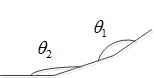
\includegraphics[width=0.2\textwidth]{./figures/angles_1}
        }
        \subfloat[sequence 2]{
           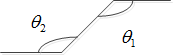
\includegraphics[width=0.2\textwidth]{./figures/angles_2}
        }        
    \end{center}
    \caption{A graphical representation of the angles of a sequence. It can be seen that per our definition Sequence 1 Complexity measure is smaller than sequence 2 complexity measure.}
   \label{fig:sequence_complexity}
\end{figure}

\section{The ADAB Database}
\label{sec:database}
The data is one of the most important part of any supervised learning technique. The data is used for learning, validation and testing. It has a critical effect on the system performance. In this work we have chosen to use the ADAB database. The ADAB database is de-facto a standard in the on-line Arabic handwriting recognition research field. It is freely available and consists of more than 20k Arabic handwritten words scribed by more than 170 different writers. The words are taken from the 937 Tunisian town/village names. It contains the trajectory information and a plot image of the word trajectory. A sample can contain more than a word. In figure \ref{fig:sample_parts} we show the parts of a sample. The ADAB database v.1 is divided to 3 sets. Details about the number of files, words, characters, and writers are given in \cite{el2009icdar}. Our training, validation and testing set both are taken from this database. 
No information relating the strokes to letters or to word-parts is provided, thus, extra work was needed to add this information to the database so that it could be used as letters samples source and also a ground-truth for the segmentation abilities of the system. To provide this additional information, we have created a system that reads the samples from the ADAB database, and employ the skills of a human expert to segment the samples and relate each stroke to the corresponding letter in the WP. The resulted information was saved in an xml file for each word sample. Since additional strokes are not our interest in the segmentation process, the system has automatically filtered out additional strokes. Nevertheless, the human expert had the ability to filter out additional strokes that could not be identified by the system as such. We have manually segmented ~16k samples which consisted about ~40k strokes. 

\begin{figure}
\centering
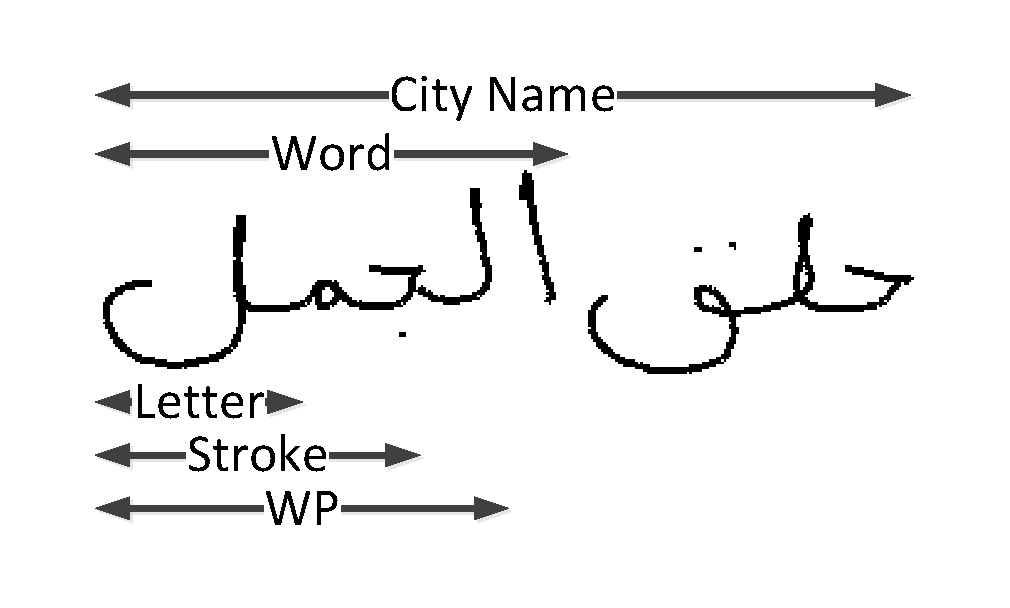
\includegraphics[width=6cm]{./figures/sample_parts}
\caption{Visual demonstration of a test sample parts.}
\label{fig:sample_parts}
\end{figure}

\section{Experimental Results}
\label{sec:results}
This section provides all the relevant experimental results that were conducted by using the proposed technique. In order to simulate the the continuous writing process of the stroke, points of the trajectory were inputed to the system one at a time. Our system is implemented using the Matlab environment. Comparing the performance of our approach to other works done in the field is not a simple task. The complexity of such task is not only the different experimental settings, databases and methodology but also the different parameters that are used to display the work results. For this reason, to make our results more clear we have chosen to display our results from two points of view. The first is the WP and the second is the segmentation point. For the WP, we have measured the Segmentation rate (SR) and the Recognition rate (RR). A Segmentation point can be considered one of the following: 1. Valid (true positive): the segmentation point is identified in the correct location. 2. Invalid (false positive): the segmentation point was identified in an incorrect place. 3. Missing: No segmentation point was identified between two successive letters.
The large test sample and the usage of the ADAB database and not a own collected database give our results further firmness. In table \ref{table:general_stats} we provide basic statistics of our sample set. We made sure that the samples taken to extract letters samples for the training of the scoring system were not used in the sample set.

\begin{table}[h]
\caption{General statistics}
\begin{tabular}{ | c | c | }
  \hline
  Number of samples (city name) & 319 \\
  \hline
  Number of WPs & 1148 \\
  \hline
  Number of Strokes & 1237 \\
  \hline
\end{tabular}
\centering
\label{table:general_stats} 
\end{table}

A correctly segmented stroke is the case when all the letters in the stroke are correctly segmented. A correct segmentation of a WP means that all the strokes of the in it were segmented correctly. The segmentation was validated by a human expert.

The results shown in table \ref{table:wp_results} summarizes the system performance in the WP level and in table \ref{table:sp_results} we provide experimental results in the segmentation points level. It is apparent that the results are promising by the high WP segmentation rate and the high precision and recall values.

\begin{table}[h]
\caption{WP Results}
\begin{tabular}{ | c | c | }
  \hline
  Segmentation Rate &  83\% \\ 
 \hline
  Recognition Rate &  78\% \\ 
 \hline
  Average Time & 0.64 [sec] \\
\hline
\end{tabular}
\centering
\label{table:wp_results} 
\end{table}

\begin{figure}
\centering
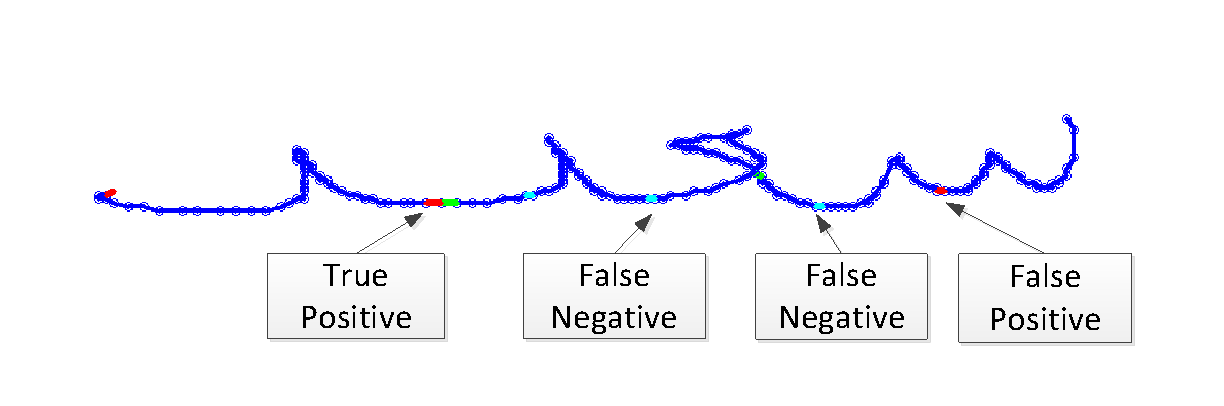
\includegraphics[width=8cm]{./figures/sp_types}
\caption{Segmentation points types. As described in figure \ref{fig:candidate_in_no_horizontal}, the cyan points indicate candidate segmentation points that were nominated but not selected by the Selection algorithms. The red points indicate the final segmentation points set.}
\label{fig:sp_types}
\end{figure}

\begin{table}[h]
\caption{Segmentation Points Results}
\begin{tabular}{ | c | c | }
  \hline
  Total number of Segmentation point & 1081 \\
  \hline
  Valid SP (True Positive) & 922 \\
  \hline
  Invalid SP (False Positive) & 119 \\
  \hline
  Missing SP (False Negative) & 159 \\
  \hline                                    
  Precision & 88.6\% \\ 
 \hline
  Recall &  85.3\% \\ 
 \hline
\end{tabular}
\centering
\label{table:sp_results} 
\end{table}

The absolute majority of the false negative segmentation points were nominated to be a candidate points. A small number were filtered out in the filtering phase but most of them were not selected by the SSA. Thus, to achieve the best results we have developed and combined several segmentation selection approaches.

\subsection{Analysis}
In this section we will discuss some common cases which were not segmented correctly. In part of these cases we did find solutions and some cases were left for future studies to face. 
\subsubsection{Over-segmentation}
In order to avoid a candidate point nomination in a HF at the beginning of the stroke which is in most cases a false candidate point, we have added the following limitation: A CP is nominated only if the sub-stroke that spans from the beginning of the stroke to the CP is complex.
In figure \ref{fig:oversegmentation_begin} we examples of such cases.

\begin{figure}[h]
\centering
        \subfloat[]{
            \label{fig:letters_same_body_1}
            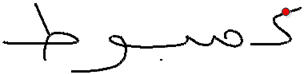
\includegraphics[width=0.3\textwidth]{./figures/oversegmentation_begin_1}
        }
        \subfloat[]{
           \label{fig:letters_same_body_2}
           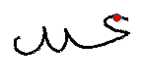
\includegraphics[width=0.15\textwidth]{./figures/oversegmentation_begin_2}
        }        
    \caption{Samples of redundant Candidate point at the beginning of the stroke.}
   \label{fig:oversegmentation_begin}
\end{figure}

Without the additional strokes, there is no way to differentiate between the main body of the letter \RL{-s-} (S) and the main body of two consecutive \RL{-b-} (B) (or other identical main body letters as seen in figure \ref{fig:same_body_letters}). See figure \ref{fig:oversegmentation_s}.  

\begin{figure}
\centering
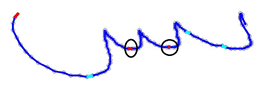
\includegraphics[width=5cm]{./figures/oversegmentation_s}
\caption{Over-segmentation in the letter \RL{-s-}. These happens since this letter is very similar to the appearance to a combination of two consecutive \RL{-b-} letters and only can be identified from the context and using the additional strokes.}
\label{fig:oversegmentation_s}
\end{figure}

We have noticed that our system tends to over-segment the letter \RL{-m-} when written in the form seen in figure \ref{fig:oversegmentation_m}. The reason for that the SSA includes the two CPs in the final segmentation set is that the letter in this form can be seen as a combination of a very frequent form of the letter \RL{-m-} and the letter \RL{-b-}. This issue can be solved by enhancing the filtering phase to eliminate CPs that are found in a loop.  

\begin{figure}
\centering
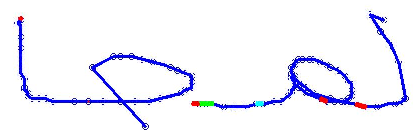
\includegraphics[width=5cm]{./figures/oversegmentation_m}
\caption{Over-segmentation appeared frequently in the letter \RL{-m}, since it contains two horizontal segments (can be handled by elimination candidate points in a loop which will be handled in future a work).}
\label{fig:oversegmentation_m}
\end{figure}

Over segmentation can be caused also from typing a letter in unusual form where it is spanned over several strokes. It happens mostly in the letter forms \RL{-m-}, \RL{-m} and in rare cases in the letter \RL{-.h-} as can be seen in figure \ref{fig:multiple_strokes_letter}.

\begin{figure}[h]
\centering
        \subfloat[]{
        		\label{fig:2_strokes_m}
            	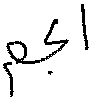
\includegraphics[width=0.1\textwidth]{./figures/2_strokes_m}
        }
        \subfloat[]{
        		\label{fig:2_strokes_7}
           	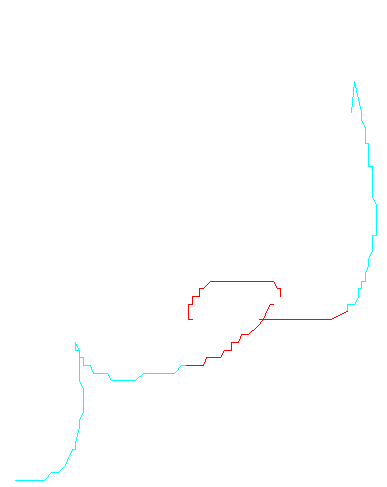
\includegraphics[width=0.1\textwidth]{./figures/2_strokes_7}
        }        
    \caption{Samples of writing a single letter using more than a single strokes. In \ref{fig:2_strokes_m} the final form of the letter \RL{m} is written in two strokes and in \ref{fig:2_strokes_7} the letter \RL{.h} is written using two strokes. These forms are less widespread.}
   \label{fig:multiple_strokes_letter}
\end{figure}

\subsubsection{Under-segmentation}
Under-segmentation may results mainly in two cases:
\begin{enumerate}
\item No candidate point is get nominated in the HF.
\item Candidate point is nominated but not selected by the SSA.
\end{enumerate}

The first mainly results from letter pairs that do not contain horizontal joint between them; this issue is partially solved by extending the notion of a letters to include such pairs of letters. For example the pair \RL{lm} and \RL{l.h}, these letters may have 2-4 positions. \\

The second may result from nomination of a candidate point on correct horizontal segment but in a late fraction of the segmentation fragment which result in a low scoring and thus not being selected by the SSA. This issue usually occurs in the letter \RL{w} in its final position (Figure \ref{fig:undersegmentation_w}).

\begin{figure}[h]
\centering
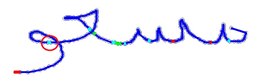
\includegraphics[width=5cm]{./figures/undersegmentation_w}
\caption{An example of a late candidate point in the letter \RL{w}.}
\label{fig:undersegmentation_w}
\end{figure}


\subsection{Sample set size}
Our letters sample set contains all letters in all its possible positions. Some letters are more frequent and more in use in general in the Arabic language, in general and in the ADAB database in particular. Thus our sample set of letters is not balanced.
On the one hand it is an advantage since the letters underlying distribution will reflect the priory probability of a letter form appearance.
On the other hand, When the imbalance gets too much big, it may negatively affect the recognition results or if allowing more samples in an imbalanced manner it may not improve the recognition results.
In the following experiment we allowed an increasing maximal number of samples per a letter position to see the affect on the segmentation and recognition rates of the system as well as on its time performance. Increasing the maximal number of samples per class (letter position) increases the imbalance between the classes. The graph in figure \ref{fig:num_letter_impact} shows that the maximal number of letters does not affect much the segmentation rate and recognition rate. The graph convergences after 200 samples per letter.  It is also evident that there is a point where allowing more samples per class may decrease the accuracy of the system.

\begin{figure}[h]
\centering
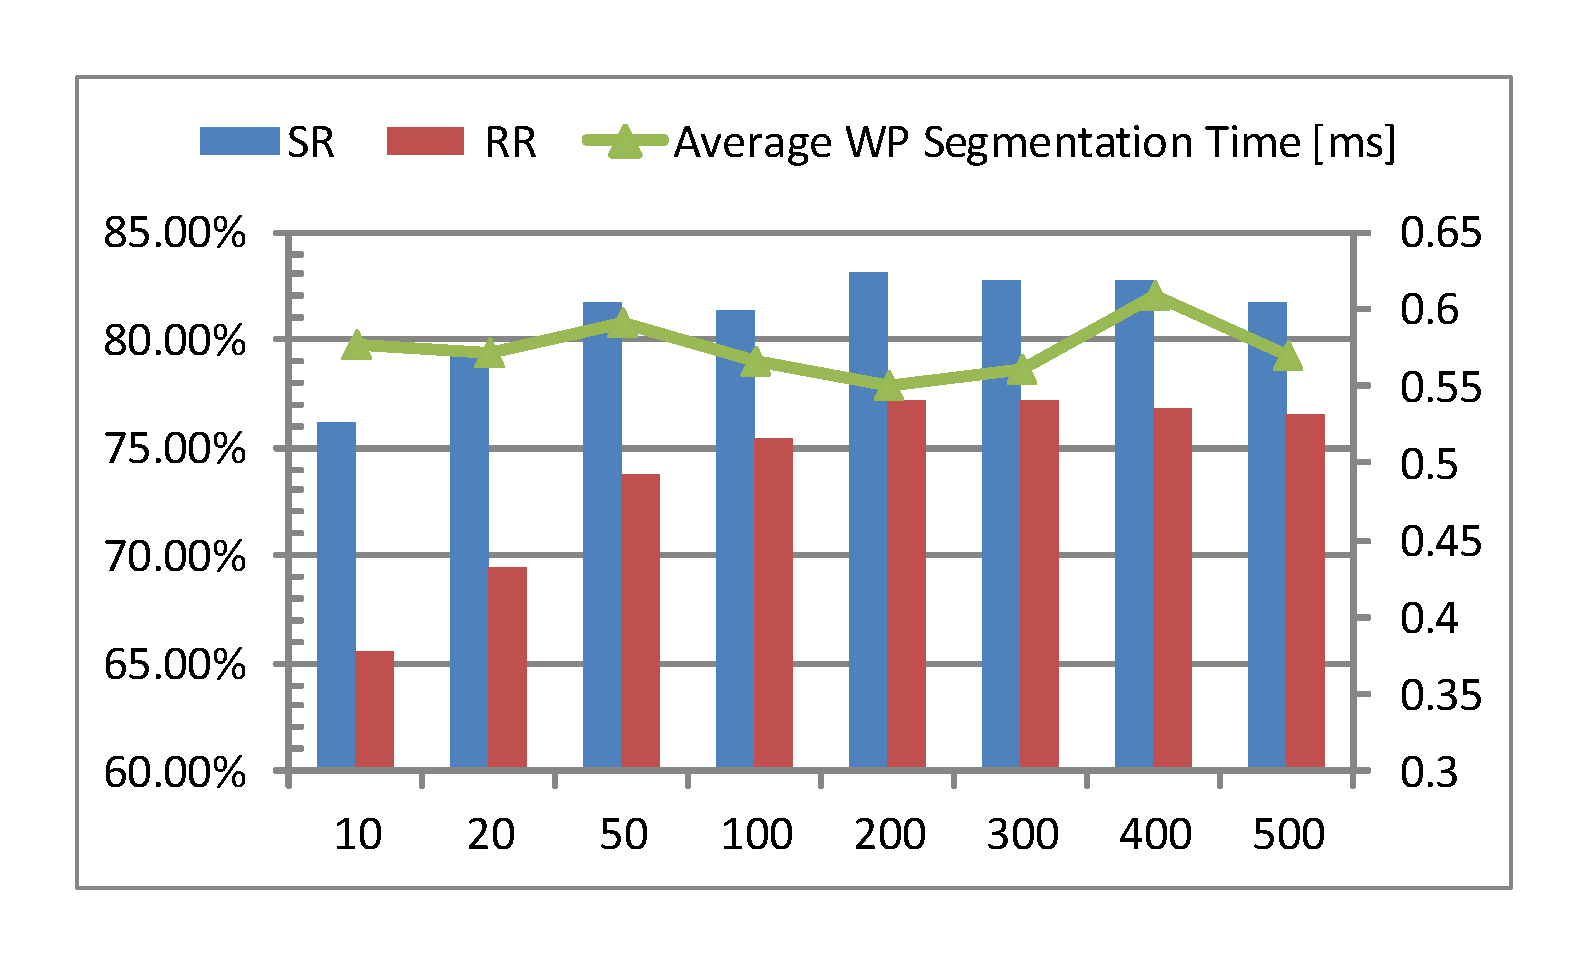
\includegraphics[width=9cm]{./figures/num_letter_impact}
\caption{The diagram shows the influence of the number of letters samples on the segmentation (SR) , recognition rates (RR) , and the average segmentation time. All the three parameters showing convergence when the maximum letter samples per letter position is larger than 200. }
\label{fig:num_letter_impact}
\end{figure}


\subsection{Segmentation Selection Algorithms performance}
\label{subsec:ssa_performance}
As can be seen in table \ref{table:ss_algorithms_results} the SSA has a crucial affect on the system performance. We tried to combine two SSA by running both SSA and select the segmentation with the smallest scoring divided by the size of $FSP$ to prevent giving superiority to segmentations with less segmentation points. Combination of two algorithms is symboled by $\oplus$.

\begin{table}[h]
\caption{SSA Performance}
\begin{tabular}{ | c | c | c | c | c |}
\hline
SSA & WP SR & WP RR & SP Precision & SP Recall\\
\hline                 
  FSS & 76\% & 70\% & 85\% & 78\% \\ 
  \hline
  BSS & 79\% &  73\% & 84\%& 81\% \\
  \hline
  BFSS & 78\% & 72\% & 84\% & 80\%\\ 
  \hline
  GSS & 80\% & 74\% & 81\% & \bf{94}\% \\  
  \hline
  FSS$\oplus$BSS & \bf{82}\% & \bf{76}\% & \bf{89}\% & 82\%\\  
  \hline
  GSS$\oplus$BFSS & 81\% & 75\% & 83\% & 90\% \\
  \hline
\end{tabular}
\centering
\label{table:ss_algorithms_results} 
\end{table}

\emph{
Handle the following:
\begin{itemize}
	\item Show how many segmentation points were found in the nomination stage. We would like to show that every real segmentation point was found at least one time in the nomination stage.
	\item Effectiveness and accuracy of the filtering stage. show how many segmentation point were filtered out in the filtering.
	\item See table 3 in \cite{eraqi2012new}, if our results are better or close to the best results, this table can be added.
	\item show some images of correctly segmented words.
	\item statistics in the stroke level.
\end{itemize}
}



\section{Future Work}
\label{sec:future_work}
\emph{[we can fix the orientation problem in figure work by rotating by different angles but the ADAB sample are our system could easily handle samples to]}

\emph{[A scoring segmentation point probability techniques can be used to identify the more probable segmentation points]}.

\emph{[Consider the delayed strokes segmentation: every strokes is classified to be in the main body or an additional stroke, id classified in the main body, then we handled it. If classified as a delayed stroke, it should be matched to the letter is related]}.

For every word, the key a serious of features such that

(A,Ham, KL): أكل
(D,Dot,HB): ذهب


\bibliographystyle{IEEEtran}
\bibliography{IEEEabrv,bibliography}

\end{document}


